\documentclass[11pt]{article}
\usepackage[margin=1in]{geometry}
\usepackage{amsmath,amssymb}
\usepackage{natbib}
\usepackage{graphicx}
\usepackage{booktabs}
\usepackage[font=small,labelfont=bf]{caption}
\usepackage{xcolor}
\usepackage[colorlinks=true,allcolors=blue]{hyperref}
\setlength{\emergencystretch}{3em}
\renewcommand{\r}{\langle r\rangle}

\title{\bfseries The consecutive spacing--ratio of nucleosome arrays:\\
high regularity from steric renewal, not level repulsion}
\author{Ruqing Chen\\[2pt]
\small GUT Geoservice Inc., Montr\'eal, Qu\'ebec, Canada\\
\small \texttt{ruqing.chen@gutgeoservice.com}}
\date{\today}

\begin{document}
\maketitle

\begin{abstract}
\noindent
Genome--wide maps place nucleosome dyads in arrays with a characteristic
$\sim$150--165\,bp repeat, and nucleosome spacing, phasing and periodicity have
been studied exhaustively. Here we examine these arrays with a statistic
borrowed from random--matrix theory (RMT): the unfold--free consecutive
spacing ratio $\r$, which discriminates uncorrelated (Poisson, $\r=0.386$),
level--repulsive (Gaussian orthogonal/unitary ensembles, $0.531/0.603$) and
rigidly regular ($\r\!\to\!1$) sequences without spectral unfolding. Applied to
base--pair--resolution chemical maps of \textit{Saccharomyces cerevisiae} and
\textit{Schizosaccharomyces pombe}, the dyad arrays give $\r\approx0.78$ and
$0.81$ --- far above every RMT ensemble, superficially suggesting strong order.
A permutation test overturns this reading: randomising the order of consecutive
linker lengths leaves $\r$ unchanged (within $0.001$), and the lag--1 spacing
autocorrelation is $\approx0$. The elevated $\r$ is therefore entirely a
property of the marginal linker--length distribution --- a steric hard--core
renewal process --- with no sequential level repulsion or spectral rigidity.
The result is robust to confidence thresholds and to nucleosome--free--region
trimming, and holds in both species, with $\r$ tracking each species' shorter or
longer repeat length. Superposing independent arrays, or randomly thinning a
single array, both drive $\r$ back toward the Poisson value, confirming that the
order is local and steric. A high spacing ratio in a genomic (or spatial) point
pattern thus need not indicate level repulsion: the permutation test is a
necessary control.
\end{abstract}

\section{Introduction}

In eukaryotes, genomic DNA is packaged into nucleosomes, each wrapping
$\sim$147\,bp of DNA around a histone octamer, separated by short linkers into
arrays with a nucleosome repeat length (NRL) of $\sim$150--200\,bp depending on
organism and chromatin context. The advent of base--pair--resolution chemical
mapping \citep{brogaard2012,moyle2013} fixed the centre (dyad) of individual
nucleosomes directly, superseding the indirect, lower--resolution micrococcal
nuclease assays. These maps established that nucleosomes occupy preferred
positions separated by near--integral multiples of the DNA helical repeat, and
that much of the genome--wide positioning is explained by steric exclusion: a
hard--core ``statistical positioning'' in which an array is set by a barrier and
the finite footprint of the particles \citep{kornberg1988,chereji2018}. Spacing
distributions, phasograms, autocorrelation functions and Fourier periodicities
of these arrays have since been characterised in great detail.

A complementary and, to our knowledge, previously unused lens on an ordered
sequence is the spectral statistics of random--matrix theory (RMT). The spacings
between consecutive levels of a sequence carry information about the underlying
process: an uncorrelated (or superposed) sequence follows Poisson statistics,
whereas a sequence with \emph{level repulsion} --- spacings that avoid small
values and are sequentially anti--correlated --- follows the Wigner--Dyson
statistics of the Gaussian ensembles \citep{bohigas1984,berry1977,mehta2004}. A
convenient, unfolding--free measure is the ratio of consecutive spacings
\citep{oganesyan2007,atas2013},
\begin{equation}
r_i=\frac{\min(s_i,s_{i+1})}{\max(s_i,s_{i+1})},\qquad s_i=x_{i+1}-x_i,
\label{eq:r}
\end{equation}
whose mean $\r$ takes the reference values $0.386$ (Poisson), $0.531$ (Gaussian
orthogonal ensemble, GOE), and $0.603$ (Gaussian unitary ensemble, GUE), and
tends to $1$ for a perfectly regular ``picket--fence'' sequence. Because
$\r$ uses only ratios of adjacent gaps it requires no spectral unfolding,
making it well suited to inhomogeneous empirical sequences.

A point that is essential below: $\r$ is \emph{two--ended}. The Poisson value
$0.386$ is the limit of an \emph{uncorrelated} (or superposed) sequence; it is
not the value of a single, clean, regular sequence, which instead tends toward
$1$. A large $\r$ can therefore arise in two very different ways --- from genuine
sequential level repulsion (as in a chaotic quantum spectrum) or, trivially,
from a narrow marginal spacing distribution with no sequential structure at all.
Distinguishing the two requires a control that destroys sequential order while
preserving the marginal: a permutation (shuffle) test.

Here we compute $\r$ for nucleosome dyad arrays for the first time, using the
high--resolution chemical maps of \textit{S.\ cerevisiae} \citep{brogaard2012}
and \textit{S.\ pombe} \citep{moyle2013}, and ask where the arrays fall and,
critically, whether any departure from Poisson reflects sequential repulsion or
merely the marginal linker distribution.

\section{Data and methods}

\paragraph{Data.} We use the published unique (distinct--nucleosome) chemical
maps: \textit{S.\ cerevisiae}, $67{,}548$ dyads on $16$ chromosomes
\citep{brogaard2012}; \textit{S.\ pombe}, $75{,}828$ dyads on $3$ chromosomes
\citep{moyle2013}. Both list, per nucleosome, a chromosome, a dyad position
(bp) and a positioning score. We deliberately use the \emph{unique} maps rather
than the accompanying ``redundant'' maps: the latter enumerate multiple
overlapping candidate positions per genomic nucleosome (median centre--to--centre
distance $\sim$12\,bp, well below the $147$\,bp footprint) and so do not
represent distinct particles; they are unsuitable for inter--nucleosome spacing.

\paragraph{Spacing ratio and permutation test.} For each chromosome we sort
dyad positions, form consecutive spacings $s_i$, and compute $\r$ from
Eq.~\eqref{eq:r}, pooling the $r_i$ within chromosomes (never across chromosome
boundaries). The \emph{shuffle test} randomly permutes the order of $\{s_i\}$
within each chromosome and recomputes $\r$. Permutation preserves the marginal
spacing distribution exactly while destroying any sequential correlation; it is
identical to drawing an i.i.d.\ renewal process from the empirical
linker--length distribution. If $\r_{\mathrm{obs}}\approx\r_{\mathrm{shuf}}$, the
value of $\r$ is set entirely by the marginal (scalar) and carries no sequential
level repulsion. We also report the lag--1 autocorrelation of the spacings,
which is clearly negative for a rigid (repulsive) spectrum and $\approx0$ for a
renewal process.

\paragraph{Superposition and thinning.} As additional diagnostics we (i)
overlay $k$ independent arrays in a shared coordinate and recompute $\r$ as a
function of $k$, and (ii) randomly thin the array (by retaining only the
highest--confidence nucleosomes) and recompute $\r$. Both operations are
expected to drive a locally--ordered sequence toward the Poisson value.

\section{Results}

\subsection{A high but shuffle--invariant spacing ratio}

For \textit{S.\ cerevisiae} the pooled spacing ratio is $\r=0.783$, essentially
identical across all $16$ chromosomes ($0.774$--$0.789$; Table~\ref{tab:main}).
This lies far above the Poisson, GOE and GUE reference values, in the
quasi--regular regime approaching the picket--fence limit
(Fig.~\ref{fig:core}a). Taken alone, the number would suggest an exceptionally
ordered sequence.

The permutation test removes this interpretation. Shuffling the order of the
linker lengths gives $\r_{\mathrm{shuf}}=0.782\pm0.0004$, differing from the
observed value by $+0.0006$ --- i.e.\ the two are indistinguishable
(Fig.~\ref{fig:core}a). The lag--1 spacing autocorrelation is $+0.05$, near zero
and, if anything, weakly positive rather than the negative value expected of a
rigid spectrum. The high $\r$ is therefore a property of the marginal spacing
distribution alone: an i.i.d.\ renewal process drawn from the same linker
distribution reproduces it exactly. There is no sequential level repulsion.

\subsection{The spacing distribution}

The origin of the high $\r$ is evident in the spacing distribution
(Fig.~\ref{fig:core}b): a sharp mode at $164$\,bp (the NRL), a hard lower edge
near the $147$\,bp nucleosome footprint (steric exclusion), a fine $\sim$10\,bp
comb from rotational positioning, and a heavy tail of large gaps from
nucleosome--free regions (NFRs) and skipped nucleosomes (overall CV $=0.61$).
The interquartile range is narrow ($147$--$187$\,bp): most consecutive spacings
are both close to the mode, so most $r_i$ are close to $1$, which is what drives
$\r$ upward. The large--gap tail inflates the coefficient of variation but
contributes only a minority of low--$r$ pairs. We note that the $\sim$10\,bp comb
and the integer--bp resolution render the spacings partly discretised rather than
drawn from a continuous density, for which the reference values of
Eq.~\eqref{eq:r} are strictly defined. This does not affect the comparison that
matters here: $\r_{\mathrm{obs}}$ and $\r_{\mathrm{shuf}}$ are computed on the
identically discretised spacings, so the shuffle test --- and hence the scalar
verdict --- is unaffected by discretisation. The permutation test is in this
sense robust to non--continuous spacing data.

\subsection{Robustness}

The scalar (shuffle--invariant) verdict is robust (Table~\ref{tab:robust}).
Excluding the large NFR gaps to isolate the bulk array raises $\r$ to
$0.81$--$0.84$ (the bulk array is an even tighter steric renewal) while leaving
$\r_{\mathrm{obs}}\approx\r_{\mathrm{shuf}}$. Conversely, randomly thinning the
array by keeping only the highest--confidence nucleosomes lowers $\r$
monotonically toward the Poisson value ($0.59\to0.48\to0.36$ for the top
$50/25/10\%$), again with $\r_{\mathrm{obs}}\approx\r_{\mathrm{shuf}}$
throughout. Random deletion of points from the array thus destroys the local
steric order and returns the sequence to Poisson --- the order is local, not a
long--range sequential property.

\subsection{Superposition drives the ratio to Poisson}

Overlaying $k$ independent arrays in a shared coordinate drives $\r$ from
$0.78$ at $k=1$ toward the Poisson value as $k$ increases
($0.78\to0.50\to0.43$ for $k=1,2,4$; Fig.~\ref{fig:core}c), for both an overlay
of distinct chromosomes and an overlay of i.i.d.\ renewals with the empirical
marginal. (The plateau slightly above $0.386$ reflects the residual hard core,
which survives superposition.) Superposition of independent ordered sequences
therefore behaves as expected for uncorrelated pooling, confirming that the
single--array order is local and additive only at the level of the marginal.
This is the well--known convergence of a superposition of independent sequences
toward Poisson statistics: the high $\r$ of a single array is a local hard--core
property rather than a long--range feature, and does not survive independent
mixing.

\subsection{Cross--species confirmation}

\textit{S.\ pombe} gives the same verdict (Fig.~\ref{fig:cross};
Table~\ref{tab:main}): $\r_{\mathrm{obs}}=0.811$, uniform across its three
chromosomes, with $\r_{\mathrm{shuf}}=0.811$ (difference $-0.0003$) and lag--1
autocorrelation $+0.07$. Its spacing distribution is shifted to shorter, tighter
values (median $151$\,bp vs.\ $164$\,bp; CV $0.47$ vs.\ $0.61$), consistent with
the species' known shorter NRL and $\sim$4--5\,bp linker preference. The
\emph{value} of $\r$ is correspondingly \emph{higher} in \textit{S.\ pombe}
(a tighter marginal yields a larger ratio), even as the scalar, non--repulsive
character is unchanged. That $\r$ shifts with the marginal exactly as the
shuffle interpretation predicts --- while the verdict remains species--invariant
--- is itself a strong internal consistency check.

\begin{table}[t]
\centering
\caption{Consecutive spacing ratio $\r$ for nucleosome dyad arrays.
Reference values: Poisson $0.386$, GOE $0.531$, GUE $0.603$, regular $\to1$.}
\label{tab:main}
\begin{tabular}{lrcccc}
\toprule
Species & $N$ pairs & $\r_{\mathrm{obs}}$ & $\r_{\mathrm{shuf}}$
 & lag--1 autocorr. & median spacing (CV)\\
\midrule
\textit{S.\ cerevisiae} & $67{,}516$ & $0.783$ & $0.782$ & $+0.05$ & $164$\,bp ($0.61$)\\
\textit{S.\ pombe}      & $75{,}825$ & $0.811$ & $0.811$ & $+0.07$ & $151$\,bp ($0.47$)\\
\bottomrule
\end{tabular}
\end{table}

\begin{table}[t]
\centering
\caption{Robustness of the shuffle--invariant verdict (\textit{S.\ cerevisiae}).
$\r_{\mathrm{obs}}\approx\r_{\mathrm{shuf}}$ throughout: the value moves with the
marginal, but the scalar (non--repulsive) character does not.}
\label{tab:robust}
\begin{tabular}{lrcc}
\toprule
Treatment & $N$ pairs & $\r_{\mathrm{obs}}$ & $\r_{\mathrm{shuf}}$\\
\midrule
all unique (baseline)              & $67{,}516$ & $0.783$ & $0.782$\\
bulk array, exclude gaps $>300$\,bp & $65{,}204$ & $0.806$ & $0.807$\\
bulk array, exclude gaps $>250$\,bp & $62{,}276$ & $0.825$ & $0.826$\\
bulk array, exclude gaps $>220$\,bp & $58{,}900$ & $0.842$ & $0.841$\\
top $50\%$ confidence (thinned)     & $33{,}750$ & $0.593$ & $0.581$\\
top $25\%$ confidence (thinned)     & $16{,}867$ & $0.480$ & $0.464$\\
top $10\%$ confidence (thinned)     & $\phantom{0}6{,}729$ & $0.358$ & $0.362$\\
\bottomrule
\end{tabular}
\end{table}

\begin{figure}[t]
\centering

\includegraphics[width=\textwidth]{nuc_fig.pdf}
\caption{Nucleosome dyad arrays in \textit{S.\ cerevisiae}.
\textbf{(a)} The observed spacing ratio ($0.783$) coincides with the shuffled
value ($0.782$) and sits far above the Poisson, GOE and GUE references:
the regularity is scalar, not level repulsion.
\textbf{(b)} Spacing distribution: a $164$\,bp mode, a hard edge near the
$147$\,bp footprint, a $\sim$10\,bp rotational comb and a large--gap (NFR) tail.
\textbf{(c)} Overlaying $k$ independent arrays drives $\r$ from $0.78$ toward the
Poisson value (real--chromosome overlay and i.i.d.\ overlay agree).}
\label{fig:core}
\end{figure}

\begin{figure}[t]
\centering
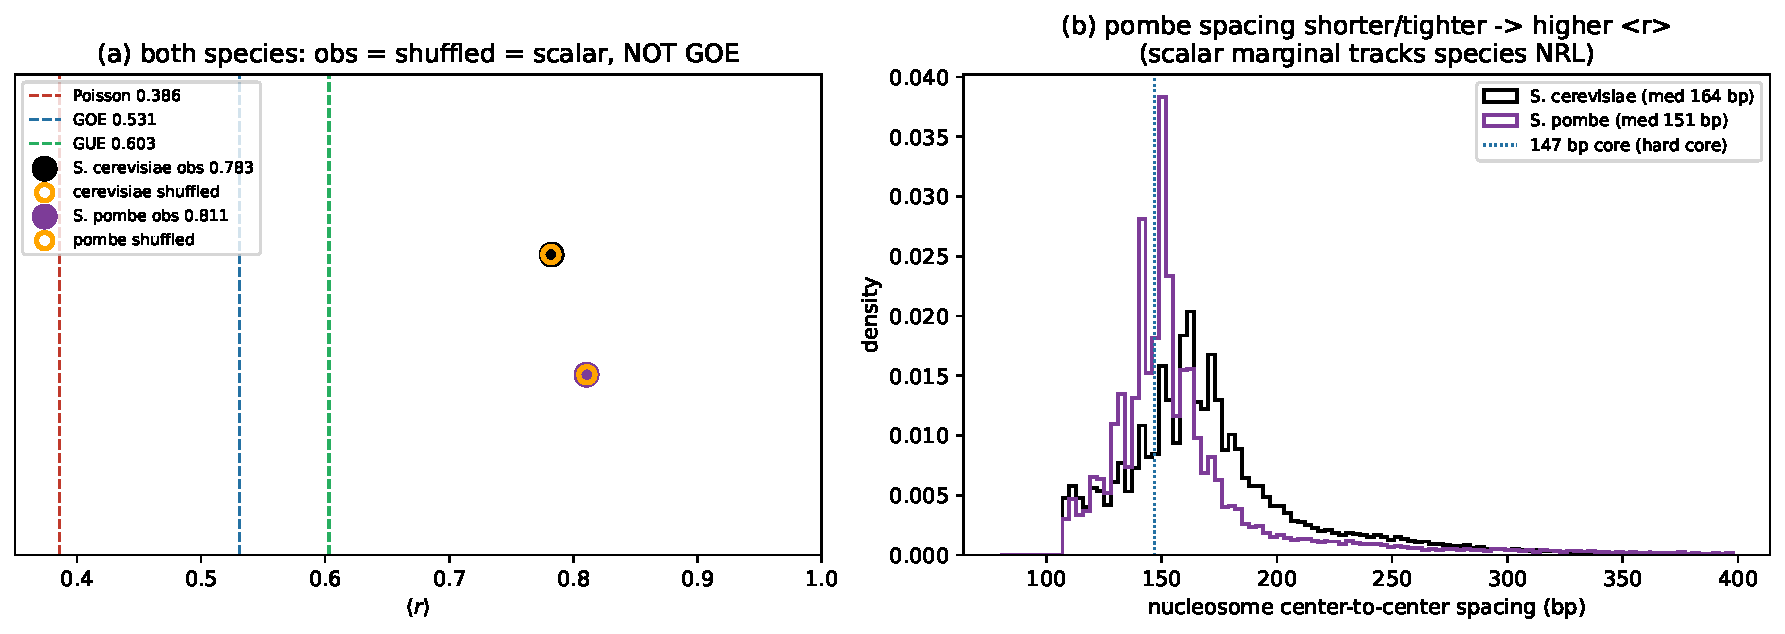
\includegraphics[width=\textwidth]{nuc_crossspecies.pdf}
\caption{Cross--species comparison.
\textbf{(a)} In both \textit{S.\ cerevisiae} and \textit{S.\ pombe} the observed
$\r$ coincides with the shuffled value (orange rings) and lies far above the RMT
ensembles --- scalar, not repulsive --- in both organisms.
\textbf{(b)} The \textit{S.\ pombe} spacing distribution is shorter and tighter
(median $151$\,bp) than \textit{S.\ cerevisiae} ($164$\,bp); the tighter marginal
yields the higher $\r$, exactly as the shuffle interpretation predicts.}
\label{fig:cross}
\end{figure}

\section{Discussion}

The consecutive spacing ratio of nucleosome dyad arrays is high
($\r\approx0.78$--$0.81$, above even the GUE value) yet entirely \emph{scalar}:
it is reproduced to three decimal places by an i.i.d.\ renewal with the same
linker--length distribution, and the spacings carry no negative sequential
correlation. The arrays are, in this precise statistical sense, a one--dimensional
steric renewal (hard--rod) process --- the quantitative signature of the
statistical--positioning and steric--occlusion pictures of nucleosome
organisation \citep{kornberg1988,chereji2018}, now expressed in the language of
level--spacing statistics. In statistical--mechanical terms the array behaves, to
first order, as a one--dimensional Tonks gas: a sequence of mutually impenetrable
hard rods of the $\sim$147\,bp footprint placed along the genome
\citep{tonks1936}. The analogy is only first order, however. An equilibrium
Tonks gas has an exponential distribution of gaps above the rod length, whereas
the observed linker distribution is sharply peaked at a preferred repeat
(Fig.~\ref{fig:core}b), indicating an additional, remodeller--set preferred
spacing superimposed on the pure steric exclusion. That extra spacing regularity
is itself scalar --- it is present, unchanged, in the shuffled sequence --- and
so likewise produces no level repulsion. A genuinely level--repulsive (Wigner--Dyson) array
would instead show $\r_{\mathrm{obs}}$ \emph{differing} from $\r_{\mathrm{shuf}}$
and a clearly negative lag--1 autocorrelation (spectral rigidity); neither is
observed.

The main methodological lesson is cautionary. Because $\r$ is two--ended, a value
far above the Poisson reference --- even above the GUE ensemble --- does not by
itself indicate order of the kind RMT describes. Here essentially all of the
elevation is marginal: it follows from a narrow, hard--core spacing distribution
and would be produced by shuffled (sequence--free) data. The permutation test is
therefore not an optional refinement but a necessary control whenever $\r$ is
applied to genomic or spatial point patterns, where narrow marginal
distributions are common. The two auxiliary diagnostics make the same point from
the opposite direction: superposing independent arrays, and randomly thinning a
single array, both return $\r$ toward Poisson, as expected when the order is
local and steric rather than a long--range sequential property.

Finally, the cross--species comparison sharpens the interpretation rather than
merely repeating it. \textit{S.\ pombe}, with its shorter repeat length and
$\sim$4--5\,bp linker preference, has a tighter marginal and correspondingly a
\emph{higher} $\r$, while the scalar, non--repulsive verdict is unchanged. The
ratio thus behaves as a faithful readout of the marginal spacing distribution
across two highly diverged genomes --- useful as a compact, unfolding--free
summary of array tightness, provided it is not over--read as level repulsion.

We emphasise what is and is not new. The regularity, periodicity and steric
basis of nucleosome spacing are well established; we claim no discovery there.
The contribution is the level--spacing--ratio (RMT) characterisation of these
arrays and the explicit demonstration --- via permutation, superposition and
thinning --- that their high $\r$ is scalar rather than repulsive. The same
toolkit, with the same controls, applies directly to other one--dimensional
genomic feature sequences.

\section*{Data availability}
\textit{S.\ cerevisiae} dyad positions: \citet{brogaard2012}, GEO accession
GSE36063 / Nature Supplementary Table~2 (unique map). \textit{S.\ pombe} dyad
positions: \citet{moyle2013}, PNAS Supporting Information Dataset~S1 (unique
map).

\paragraph{Code availability.} Analysis code, derived spacing data and figures
are openly available at
\url{https://github.com/Ruqing1963/nucleosome-spacing-ratio} and archived on
Zenodo (DOI assigned on release).

\section*{Acknowledgements}
The author thanks the laboratories of J.\ Widom and colleagues for making the
base--pair--resolution chemical maps publicly available.

\begin{thebibliography}{99}

\bibitem[Atas et al.(2013)]{atas2013}
Y.~Y. Atas, E.~Bogomolny, O.~Giraud, and G.~Roux.
Distribution of the ratio of consecutive level spacings in random matrix
ensembles. \textit{Phys. Rev. Lett.} \textbf{110}, 084101 (2013).

\bibitem[Berry \& Tabor(1977)]{berry1977}
M.~V. Berry and M.~Tabor.
Level clustering in the regular spectrum.
\textit{Proc. R. Soc. Lond. A} \textbf{356}, 375--394 (1977).

\bibitem[Bohigas et al.(1984)]{bohigas1984}
O.~Bohigas, M.~J. Giannoni, and C.~Schmit.
Characterization of chaotic quantum spectra and universality of level
fluctuation laws. \textit{Phys. Rev. Lett.} \textbf{52}, 1--4 (1984).

\bibitem[Brogaard et al.(2012)]{brogaard2012}
K.~Brogaard, L.~Xi, J.-P. Wang, and J.~Widom.
A map of nucleosome positions in yeast at base--pair resolution.
\textit{Nature} \textbf{486}, 496--501 (2012).

\bibitem[Chereji et al.(2018)]{chereji2018}
R.~V. Chereji, S.~Ramachandran, T.~D. Bryson, and S.~Henikoff.
Precise genome--wide mapping of single nucleosomes and linkers in vivo.
\textit{Genome Biol.} \textbf{19}, 19 (2018).

\bibitem[Kornberg \& Stryer(1988)]{kornberg1988}
R.~D. Kornberg and L.~Stryer.
Statistical distributions of nucleosomes: nonrandom locations by a stochastic
mechanism. \textit{Nucleic Acids Res.} \textbf{16}, 6677--6690 (1988).

\bibitem[Mehta(2004)]{mehta2004}
M.~L. Mehta. \textit{Random Matrices}, 3rd ed.
Elsevier/Academic Press, Amsterdam (2004).

\bibitem[Moyle--Heyrman et al.(2013)]{moyle2013}
G.~Moyle--Heyrman, T.~Zaichuk, L.~Xi, Q.~Zhang, O.~C. Uhlenbeck, R.~Holmgren,
J.~Widom, and J.-P. Wang.
Chemical map of \textit{Schizosaccharomyces pombe} reveals species--specific
features in nucleosome positioning.
\textit{Proc. Natl. Acad. Sci. USA} \textbf{110}, 20158--20163 (2013).

\bibitem[Oganesyan \& Huse(2007)]{oganesyan2007}
V.~Oganesyan and D.~A. Huse.
Localization of interacting fermions at high temperature.
\textit{Phys. Rev. B} \textbf{75}, 155111 (2007).

\bibitem[Tonks(1936)]{tonks1936}
L.~Tonks.
The complete equation of state of one, two and three--dimensional gases of hard
elastic spheres. \textit{Phys. Rev.} \textbf{50}, 955--963 (1936).

\end{thebibliography}

\end{document}
